\chap{Chapter 6: Field Effect Transistor (FET)}

\section{Introduction}
In the Bipolar Junction Transistor  tutorials, we saw that the output Collector current of the transistor is proportional to input current flowing into the Base terminal of the device, thereby making the bipolar transistor a \textbf{CURRENT} operated device (Beta model) as a smaller current can be used to switch a larger load current.\\

The Field Effect Transistor, or simply FET however, uses the voltage that is applied to their input terminal, called the Gate to control the current flowing through them resulting in the output current being proportional to the input voltage. As their operation relies on an electric field (hence the name field effect) generated by the input Gate voltage, this then makes the Field Effect Transistor a \textbf{VOLTAGE} operated device.\\

The Field Effect Transistor has one major advantage over its standard bipolar transistor cousins, in that their input impedance, (Rin) is very high, (thousands of Ohms), while the BJT is comparatively low. This very high input impedance makes them very sensitive to input voltage signals, but the price of this high sensitivity also means that they can be easily damaged by static electricity.

\section{Junction Field Effect Transistor}
We saw previously that a bipolar junction transistor is constructed using two PN-junctions in the main current carrying path between the Emitter and the Collector terminals. The Junction Field Effect Transistor (JUGFET or JFET) has no PN-junctions but instead has a narrow piece of high resistant semiconductor material forming a “Channel” of either N-type or P-type silicon for the majority carriers to flow through with two ohmic electrical connections at either end commonly called the Drain and the Source, respectively.\\

\textbf{Before analysing the circuit using JFET, students are proposed to characterize the I-V curve of a JFET in PSPICE (named \textbf{JbreakN in the Favourite list}), to determine IDSS and VP, which are two parameters for a JFET}. The circuit bellow is required to implement in PSPICE:

\begin{figure}[!htp]
    \centering
    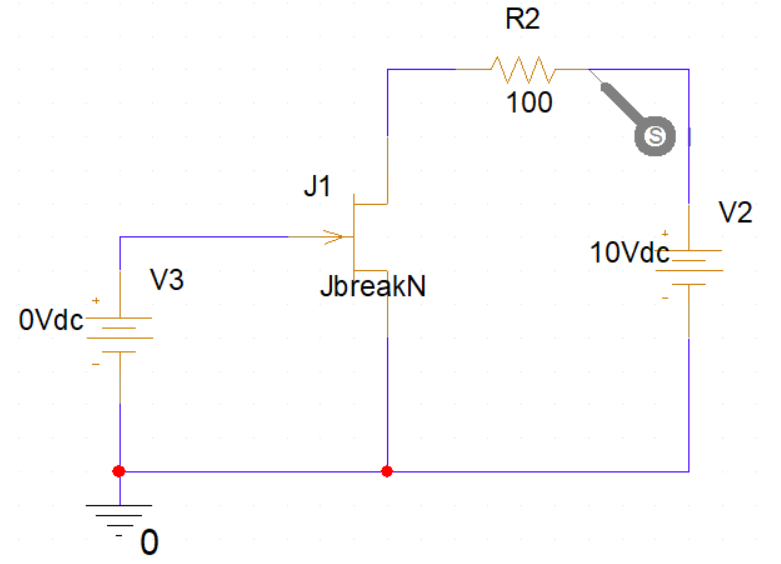
\includegraphics[width = 3.5in]{source/picture/bai_6/fet1.PNG}
    \caption{JFET circuit in PSPICE}
    \label{jfet_1}
\end{figure}

\subsection{DC Sweep simulation}
In the first simulation, a DC sweep for input source V3 is perform, varying from -3V to 0V to verify the \textbf{active region}. The simulation profile is suggested as follows:

\begin{figure}[!htp]
    \centering
    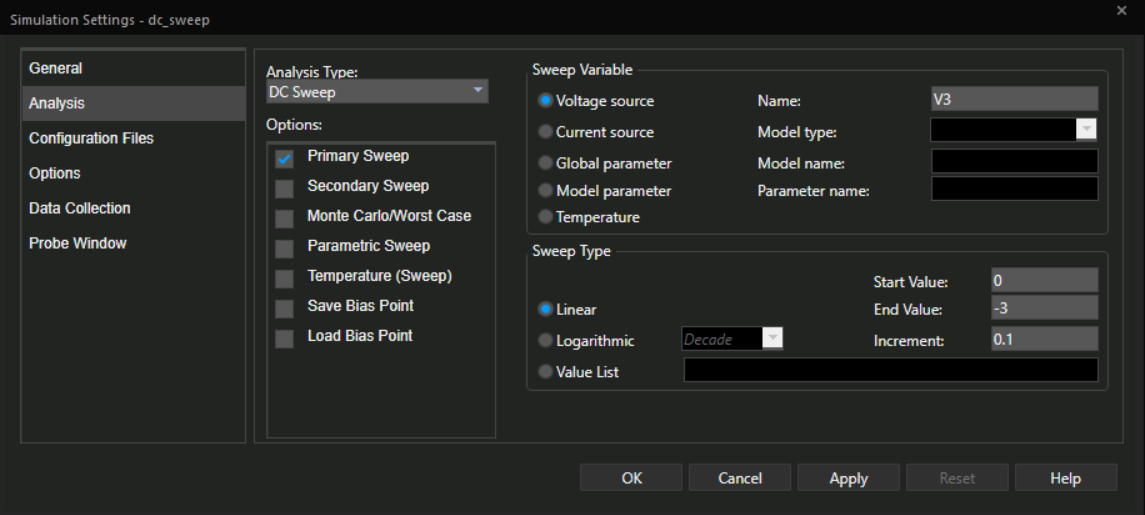
\includegraphics[width = 4in]{source/picture/bai_6/jfet2.PNG}
    \caption{DC Sweep simulation profile}
    \label{jfet_2}
\end{figure}

The simulation results are presented in the following figure:
\begin{figure}[!htp]
    \centering
    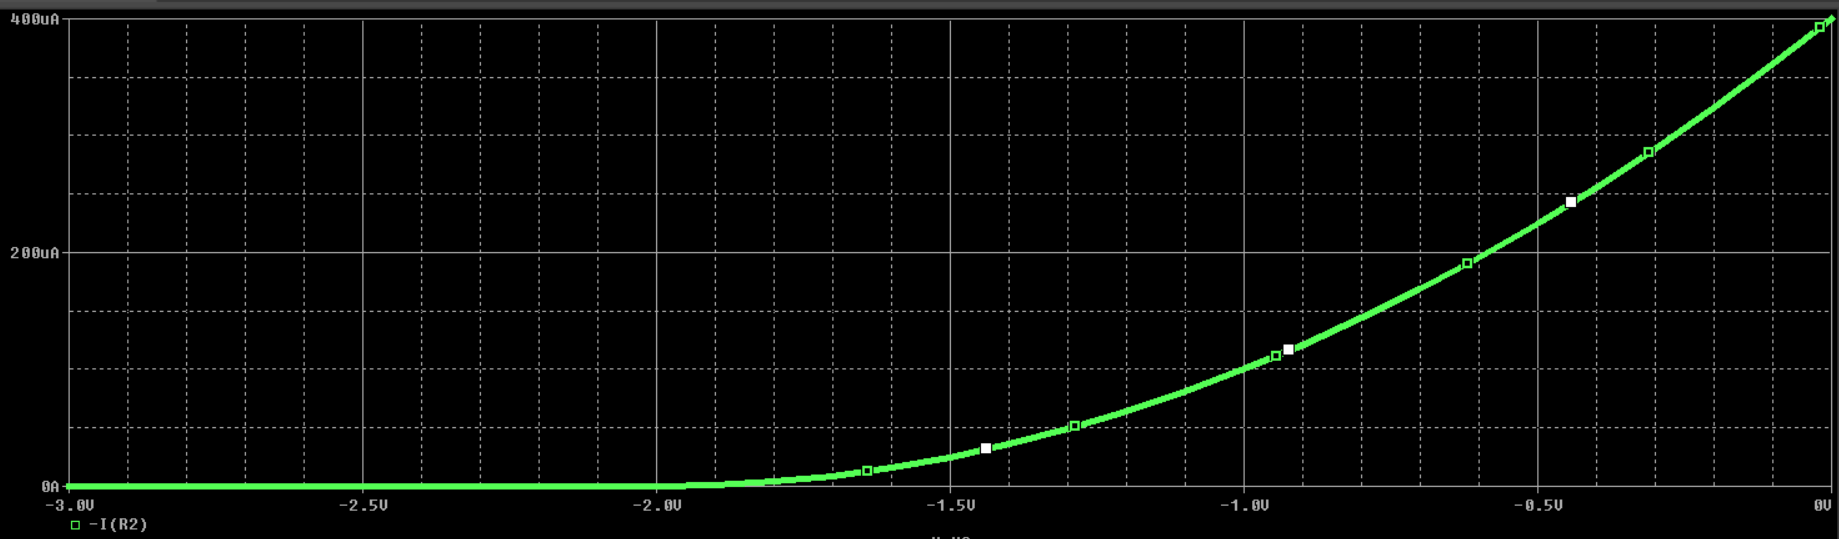
\includegraphics[width = 4in]{source/picture/bai_6/jfet3.PNG}
    \caption{Simulation results for sweeping V3 from -3V to 0V}
    \label{jfet_3}
\end{figure}

The simulation results confirm that \textbf{IDSS = 400mA} and \textbf{VP = -2V} for a typical JFET device in PSPICE.

\subsection{Nested DC Sweep simulation}
In this simulation, more details for the I-V characteristics are performed. Instead of varying the source V3, V2 can be also varied in a nested DC Sweep simulation.\\

Firstly, for the primary DC sweep source, which is set to V2, is configured as follows:
\begin{figure}[!htp]
    \centering
    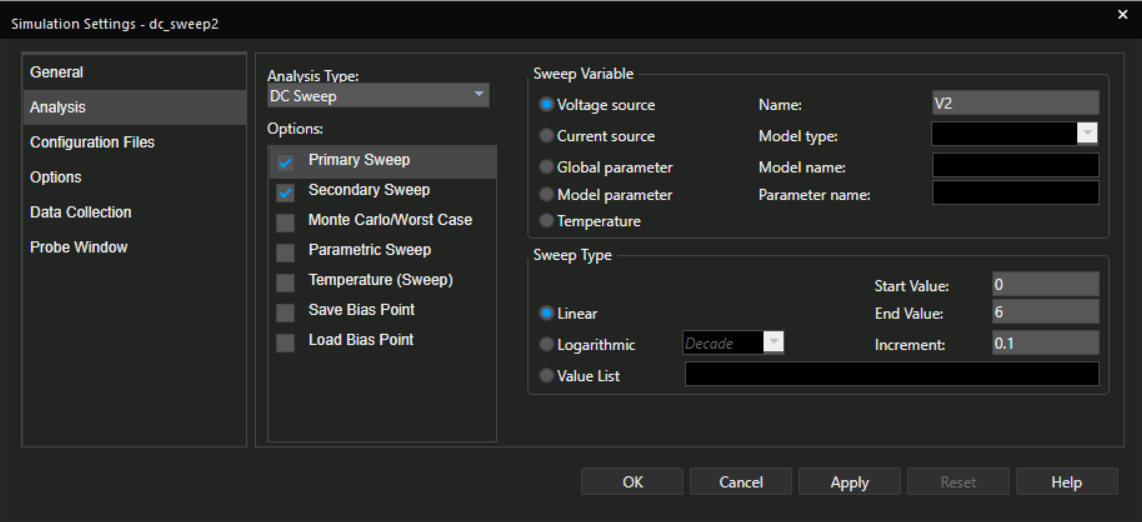
\includegraphics[width = 4.5in]{source/picture/bai_6/jfet4.PNG}
    \caption{Primary dc sweep source V2}
    \label{jfet_4}
\end{figure}

Secondly, the secondary DC sweep source, which is set to V3, is configured as follows:

\begin{figure}[!htp]
    \centering
    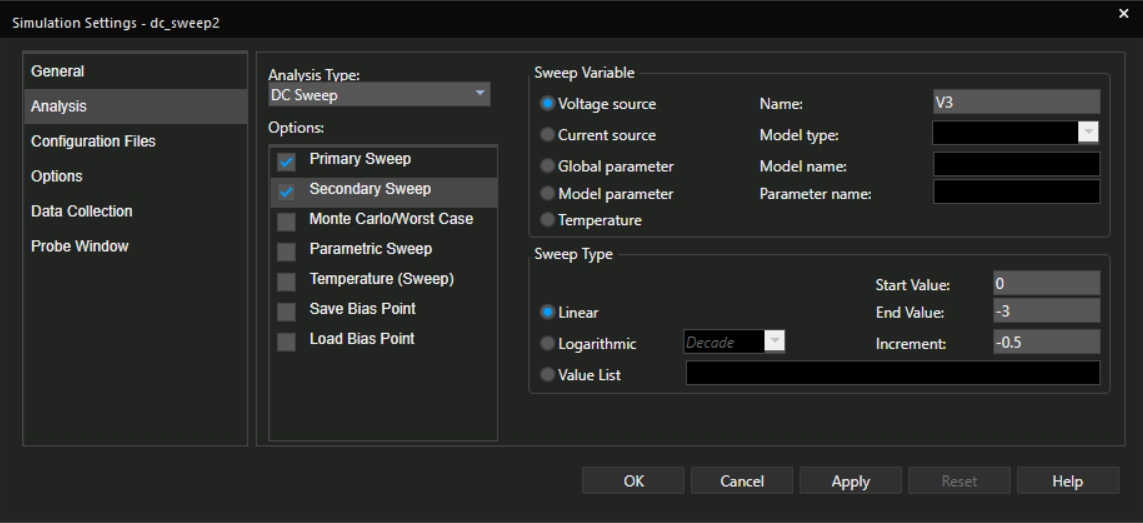
\includegraphics[width = 4.5in]{source/picture/bai_6/jfet5.PNG}
    \caption{Primary dc sweep source V3}
    \label{jfet_5}
\end{figure}

The simulation results are shown as the figure bellow:

\begin{figure}[!htp]
    \centering
    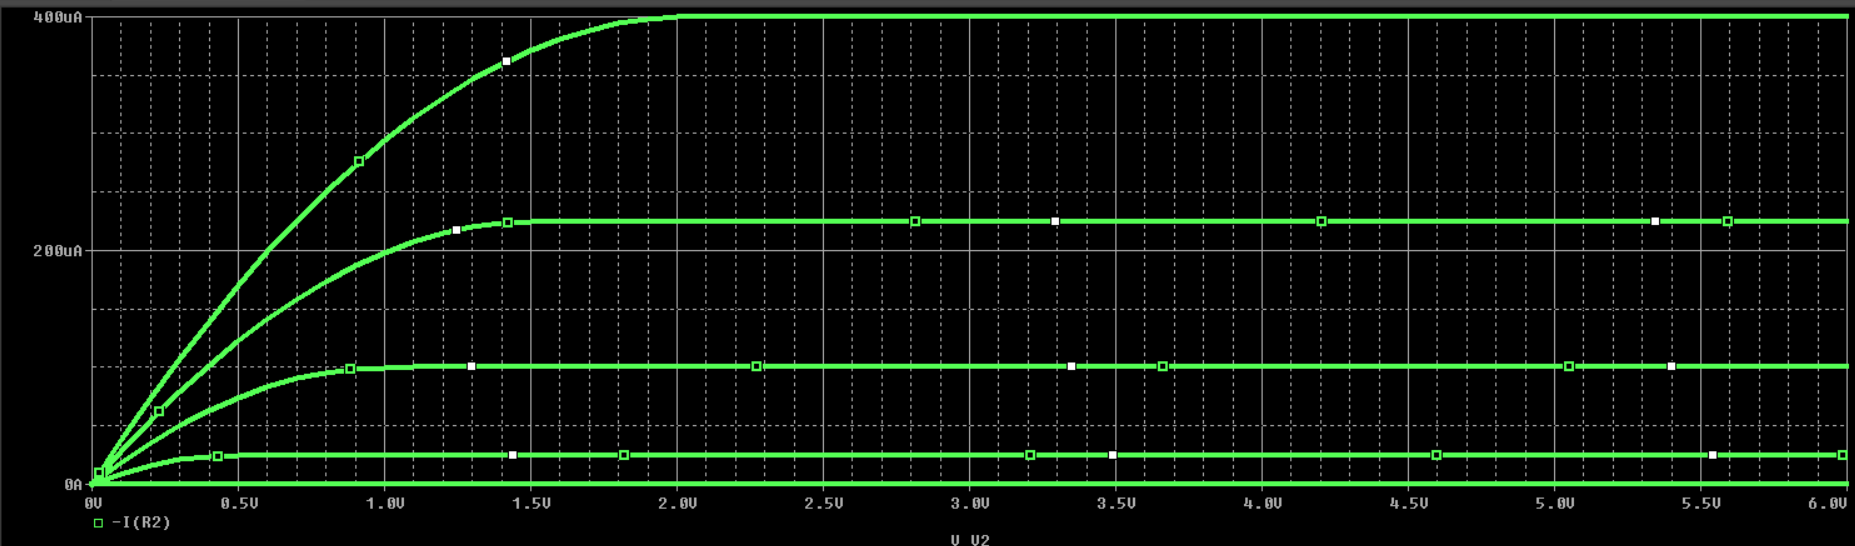
\includegraphics[width = 4.5in]{source/picture/bai_6/jfet6.PNG}
    \caption{Simulation results with JFET}
    \label{jfet_6}
\end{figure}

This figure also confirm that IDSS = 400mA and VP = -2V (the lowest curve is -1.9V). In this simulation, the ohmic region and saturation region are indicated better.

\subsection{Exercises}
\subsubsection{Self bias configuration}
This is the first configuration for a JFET, when the Gate pin is connected to the Ground. A typical circuit is presented as follows:

\begin{figure}[!htp]
    \centering
    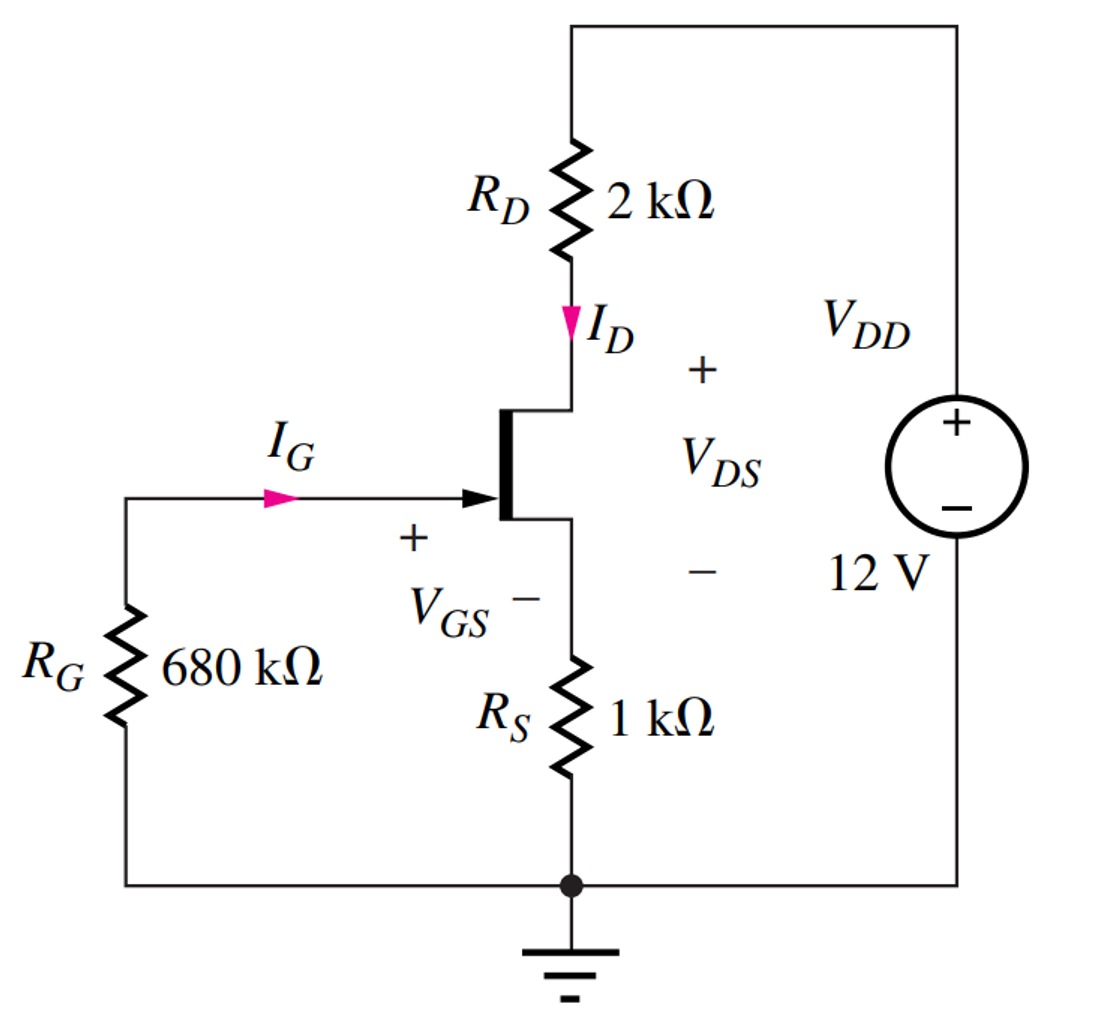
\includegraphics[width = 2.5in]{source/picture/bai_6/jfet7.PNG}
    \caption{Self bias configuration}
    \label{jfet_7}
\end{figure}

Students are proposed to implement this circuit in PSPICE with the JFET is JbreakN. The simulation results in PSPICE (\textbf{bias configuration}) are presented here. Moreover, a short explanations are required in this report to explain the value of ID and VGS.

\subsubsection{Voltage divider configuration}
The proposed schematic for this configuration is presented as follows:
\begin{figure}[!htp]
    \centering
    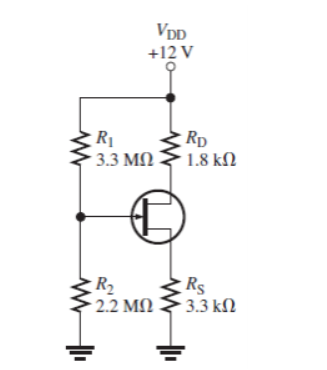
\includegraphics[width = 2.5in]{source/picture/bai_6/jfet8.PNG}
    \caption{Voltage divider configuration}
    \label{jfet_8}
\end{figure}

Students are proposed to implement this circuit in PSPICE with the JFET is JbreakN. The simulation results in PSPICE (\textbf{bias configuration}) are presented here. Moreover, a short explanations are required in this report to explain the value of ID and VGS.

\section{Metal Oxide Semiconductor FET}
As well as the Junction Field Effect Transistor (JFET), there is another type of Field Effect Transistor available whose Gate input is electrically insulated from the main current carrying channel and is therefore called an Insulated Gate Field Effect Transistor.\\

The most common type of insulated gate FET which is used in many different types of electronic circuits is called the Metal Oxide Semiconductor Field Effect Transistor or MOSFET for short.\\

The IGFET or MOSFET is a voltage controlled field effect transistor that differs from a JFET in that it has a “Metal Oxide” Gate electrode which is electrically insulated from the main semiconductor n-channel or p-channel by a very thin layer of insulating material usually silicon dioxide, commonly known as glass.

\subsection{Depletion-mode MOSFET}
The Depletion-mode MOSFET, which is less common than the enhancement mode types. This device is very similar to JFET, except that the maximum current saturation is obtained at VGS > 0.  The circuit used to verify IDSS and VP for DFET is presented as follows:

\begin{figure}[!htp]
    \centering
    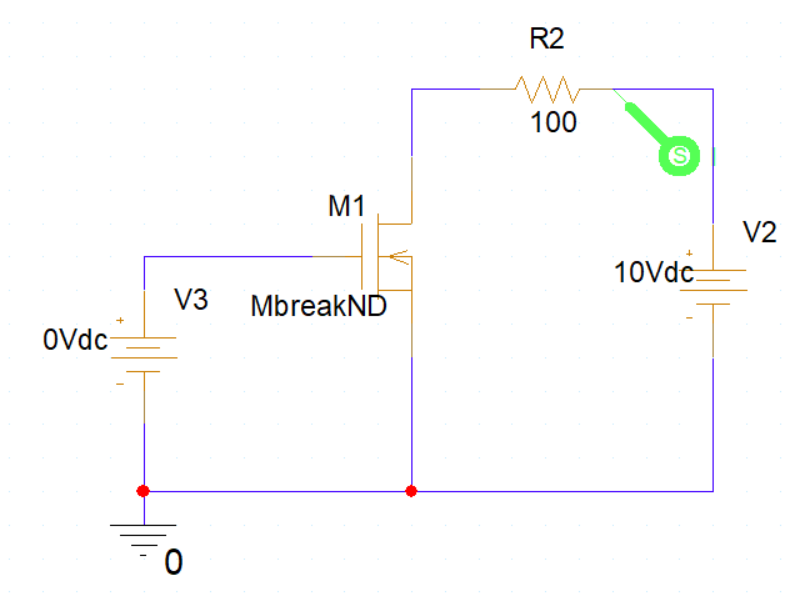
\includegraphics[width = 3in]{source/picture/bai_6/dfet1.PNG}
    \caption{DFET verification in PSPICE}
    \label{dfet_1}
\end{figure}

The device for a common DFET is MbreakND. After a dc sweep simulation when V3 varies from -5V to 0V, the results are shown bellow:

\begin{figure}[!htp]
    \centering
    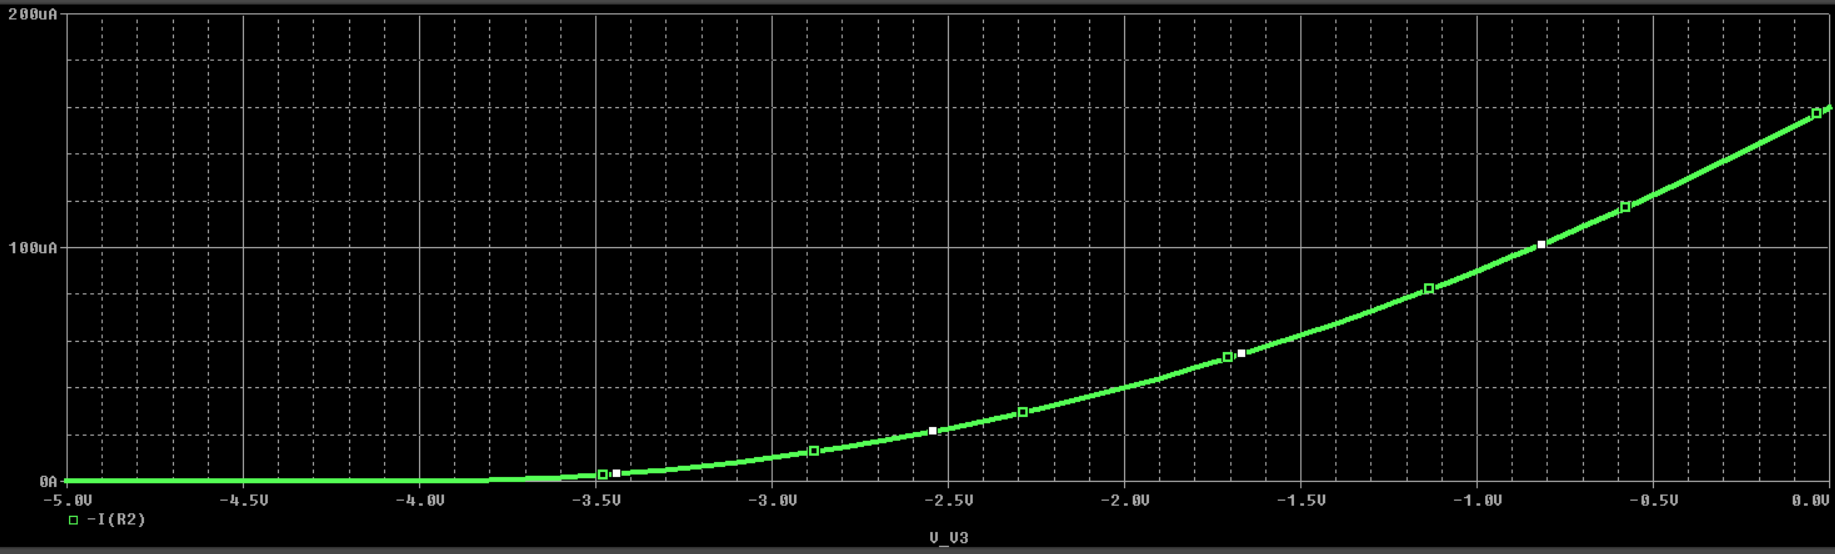
\includegraphics[width = 3in]{source/picture/bai_6/dfet2.PNG}
    \caption{Simulation results with DFET}
    \label{dfet_2}
\end{figure}

From this simulation results, it is confirmed that IDSS = 160mA and VP = -4V for DFET.\\

\textbf{Students are proposed to implement the circuit bellow:}

\begin{figure}[!htp]
    \centering
    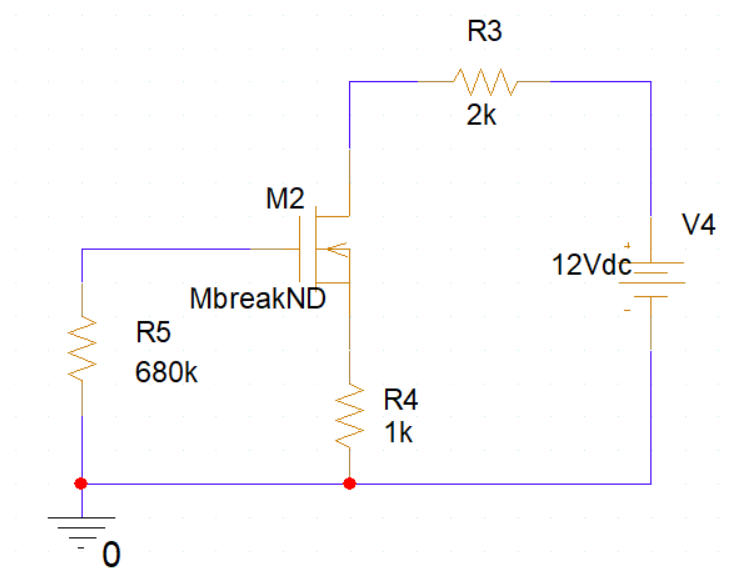
\includegraphics[width = 3in]{source/picture/bai_6/dfet3.PNG}
    \caption{Self bias configuration for DFET}
    \label{dfet_3}
\end{figure}

Only the bias configuration is required to executed. Please capture the simulation results with current and voltage information on the circuit. Finally, explain these values by theory calculations.


\subsection{Enhancement-mode MOSFET}
The more common Enhancement-mode MOSFET or eMOSFET. The device is normally “OFF” (non-conducting) when the gate bias voltage, VGS is equal to zero. For the n-channel enhancement MOS transistor a drain current will only flow when a gate voltage ( VGS ) is applied to the gate terminal greater than the threshold voltage ( VTH ) level in which conductance takes place making it a transconductance device. In other words, for an n-channel enhancement mode MOSFET: +VGS turns the transistor “ON”, while a zero or -VGS turns the transistor “OFF”. Thus the enhancement-mode MOSFET is equivalent to a “normally-open” switch.\\

The reverse is true for the p-channel enhancement MOS transistor. When VGS = 0 the device is “OFF” and the channel is open. The application of a negative (-ve) gate voltage to the p-type eMOSFET enhances the channels conductivity turning it “ON”. Then for an p-channel enhancement mode MOSFET: +VGS turns the transistor “OFF”, while -VGS turns the transistor “ON”. \\

The validation of an EFET in PSPICE is presented bellow. The typical EFET in PSPICE is \textbf{MbreakN} device.

\begin{figure}[!htp]
    \centering
    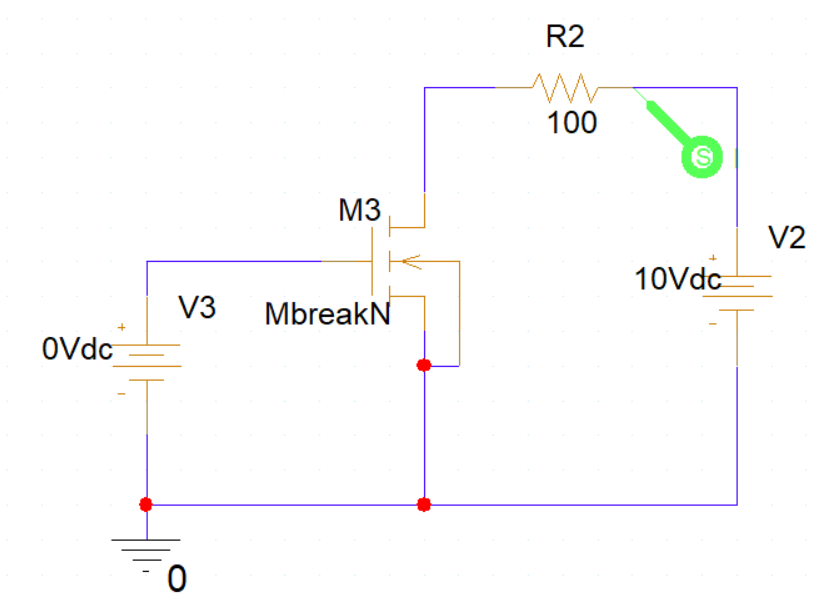
\includegraphics[width = 3in]{source/picture/bai_6/efet1.PNG}
    \caption{EFET validation}
    \label{efet_1}
\end{figure}

A dc sweep simulation with V3 can be performed. The simulation results with V3 varies from -1V to 5V are presented as following:
\begin{figure}[!htp]
    \centering
    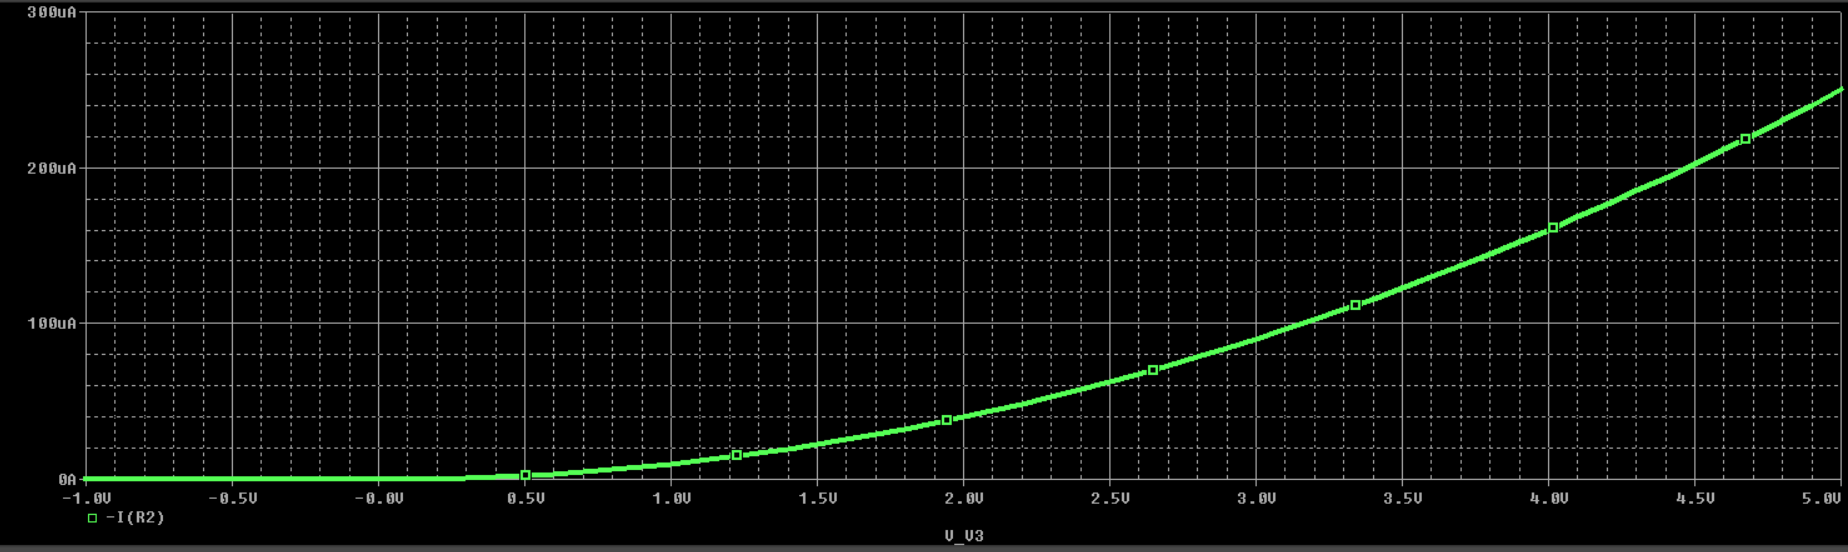
\includegraphics[width = 4.5in]{source/picture/bai_6/efet2.PNG}
    \caption{Simulation results with EFET}
    \label{efet_1}
\end{figure}

\section{MOSFET Applications}
This part presents some applications using MOSFETs and most of them are EFETs. Students are proposed to implement the schematic and then, validate in PSPICE.
\subsection{MOSFET as a switch}
In this circuit arrangement an Enhancement-mode N-channel MOSFET is being used to switch a simple lamp “ON” and “OFF” (\textbf{could be replace by an resistor to simulate in PSPICE}).

\begin{figure}[!htp]
    \centering
    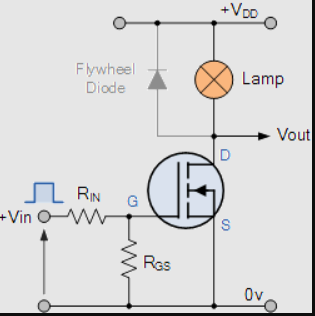
\includegraphics[width = 2.5in]{source/picture/bai_6/fet_app_1.PNG}
    \caption{EFET is used as a switch}
    \label{fet_app_1}
\end{figure}

The gate input voltage VGS is taken to an appropriate positive voltage level to turn the device and therefore the lamp load either “ON”, ( VGS = +ve ) or at a zero voltage level that turns the device “OFF”, ( VGS = 0V ).\\

If the resistive load of the lamp was to be replaced by an inductive load such as \textbf{a coil, solenoid or relay} a “flywheel diode” would be required in parallel with the load to protect the MOSFET from any self generated back-emf.\\

\textbf{Students are proposed to simulation this circuit with RIN = 4.7k and RGS = 47k and VIN is the TTL level (0V and 5V). The power supply for VDD can be set to 12V or 24V. Shortly explain the current passing through the load (a resistance 100Ohm replaced for the Lamp in the circuit)}.

\subsection{MOSFET Motor Controller [Optional]}
As the motor load is inductive, a simple flywheel diode is connected across the inductive load to dissipate any back emf generated by the motor when the MOSFET turns it “OFF”. A clamping network formed by a zener diode in series with the diode can also be used to allow for faster switching and better control of the peak reverse voltage and drop-out time.

\newpage
\begin{figure}[!htp]
    \centering
    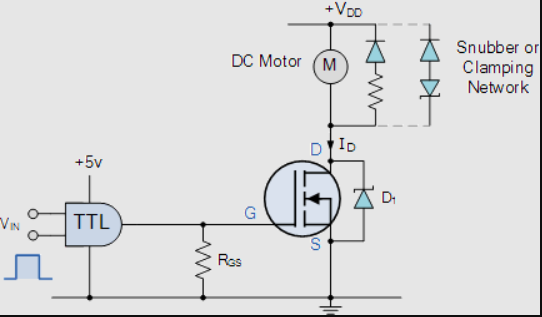
\includegraphics[width = 3in]{source/picture/bai_6/fet_app_2.PNG}
    \caption{Simple motor controller using EFET}
    \label{fet_app_2}
\end{figure}

For added security an additional silicon or zener diode D1 can also be placed across the channel of a MOSFET switch when using inductive loads, such as motors, relays, solenoids, etc, for suppressing over voltage switching transients and noise giving extra protection to the MOSFET switch if required. Resistor RGS is used as a pull-down resistor to help pull the TTL output voltage down to 0V when the MOSFET is switched “OFF”.

\textbf{This exercise is optional in this lab.}

\subsection{Complementary MOSFET Motor Controller [Optinal]}

The two MOSFETs are configured to produce a bi-directional switch from a dual supply with the motor connected between the common drain connection and ground reference. When the input is LOW the P-channel MOSFET is switched-ON as its gate-source junction is negatively biased so the motor rotates in one direction. Only the positive +VDD supply rail is used to drive the motor.

\begin{figure}[!htp]
    \centering
    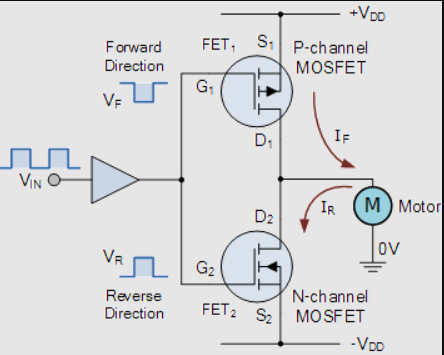
\includegraphics[width = 3.5in]{source/picture/bai_6/fet_app_3.PNG}
    \caption{Full Motor controller with N and P channel EFET}
    \label{fet_app_3}
\end{figure}

When the input is HIGH, the P-channel device switches-OFF and the N-channel device switches-ON as its gate-source junction is positively biased. The motor now rotates in the opposite direction because the motors terminal voltage has been reversed as it is now supplied by the negative -VDD supply rail.\\

Then the P-channel MOSFET is used to switch the positive supply to the motor for forward direction (high-side switching) while the N-channel MOSFET is used to switch the negative supply to the motor for reverse direction (low-side switching).\\

\textbf{This exercise is also optional in this lab.}
\section{Altium Designer}
\subsection{Button Input}
Pushbuttons or switches connect two points in a circuit when you press them. In a system, button is a traditional input method. The figure bellow is an example of a simple button, which is the target of this exercise:
\begin{figure}[!htp]
    \centering
    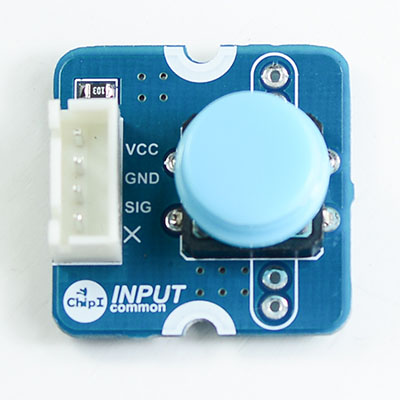
\includegraphics[width = 2in]{source/picture/bai_6/ChipI_Button.jpg}
    \caption{An example of a button}
    \label{altium_1a}
\end{figure}

The schematic of this circuit is proposed as follows:
\begin{figure}[!htp]
    \centering
    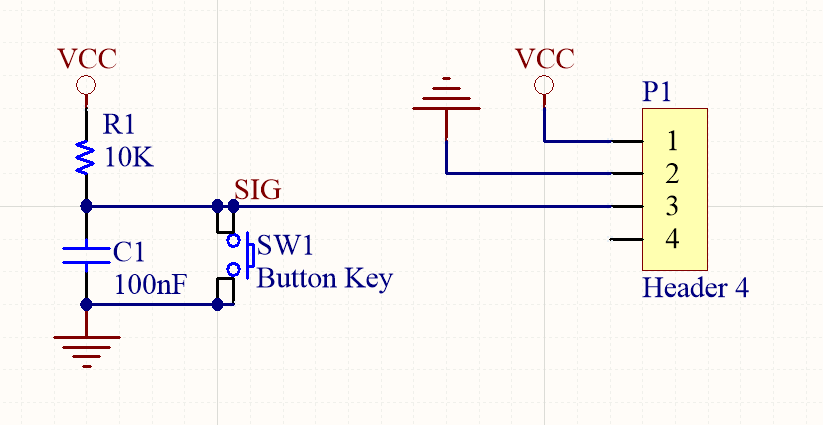
\includegraphics[width = 4in]{source/picture/bai_6/altium_1.PNG}
    \caption{Button schematic in Altium}
    \label{altium_1b}
\end{figure}

\textbf{Students are proposed to implement the circuit in Altium Designer. The manual can be found in the same playlist with other manual videos. Please capture the screen to present the schematic as well as the layout of your PCB.}

\subsection{ADC Input}
The second type of the input signal is the ADC input value, which is a kind of sensing device. In this sensor part, we use two opamps which are packed in one IC LM358. IC LM358 includes two opamps. A photoresistor (also known as a light-dependent resistor, LDR, or photo-conductive cell) is use to measure the light intensitive. It is a passive component that decreases resistance with respect to receiving luminosity (light) on the component's sensitive surface. An example of this module can be found in the figure bellow:

\begin{figure}[!htp]
    \centering
    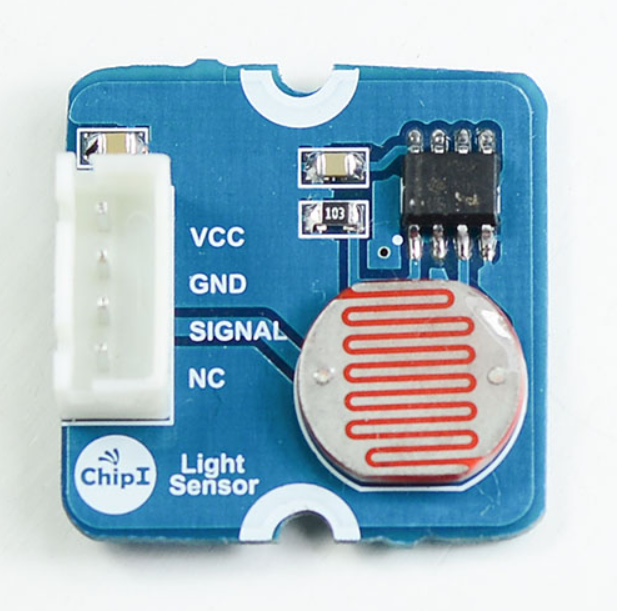
\includegraphics[width = 2in]{source/picture/bai_6/light_sensor.PNG}
    \caption{An example of a light sensor}
    \label{altium_2a}
\end{figure}

The schematic of this circuit is proposed as follows, which is based on a voltage follower circuit:
\begin{figure}[!htp]
    \centering
    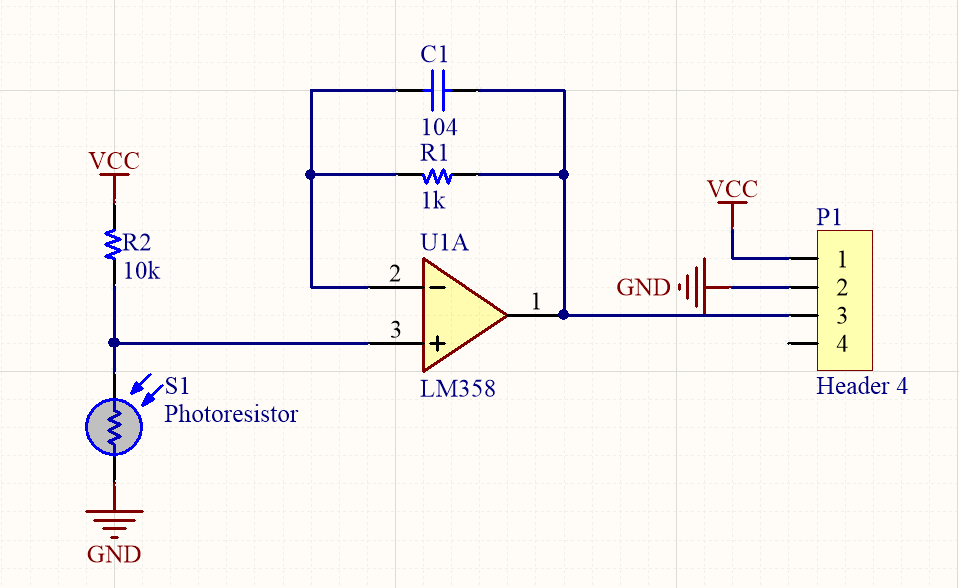
\includegraphics[width = 4in]{source/picture/bai_6/altium_2.PNG}
    \caption{Light sensor schematic in Altium}
    \label{altium_2b}
\end{figure}


\textbf{Students are proposed to implement the circuit in Altium Designer. The manual can be found in the same playlist with other manual videos. Please capture the screen to present the schematic as well as the layout of your PCB.}